

\required{Section III: Detailed Proposal Information}
\section{Statement of Work (SOW)}
The project's aim is to develop a minaturized high-sensitivity, low-noise magnetic gradiometer. Our approach is to mimic the mechanism found in magnetosomes, the specialized cells from bacteria to higher vertebrates such as fish and birds (see \ref{sec:inno}). This is comprised of three main tasks: modeling and simulation, microfabrication process design, and circuit design. Each Phase (1,2,3) will include these three tasks and is concluded with  a task on testing and analysis. No task requires the use of government equipment. 'Successful' completion of a design indicates satisfaction of the parameters in Table \ref{table:obj} following the test procedures described in \ref{sec:test}. Testing will be completed at UF by Drs. Casanova and Yoon at UF in all phases.

\begin{table}[h!]
\centering
  \begin{tabular}{|c||c|c|c|}
    \hline
     & Phase 1 & Phase 2 & Phase 3 \\
    \hline
    \hline
    Power consumption & 150 mW & 50 mW & 100 mW \\
    \hline
    Sensor Volume & 3x3x10 cm & 1x1x7 cm & 1x1x7 cm \\
    \hline
    Control Electronics Volume  & N/A & N/A & 20cm$^3$ \\
    \hline
    Ambient Magnetic Field & $\pm$ 100 $\mu$T & $\pm$ 100 $\mu$T & $\pm$ 100 $\mu$T \\
    \hline
    Ambient Operating Temperature & N/A & 0$^{\circ}$ C to 50$^{\circ}$ C & 0$^{\circ}$ C to 50$^{\circ}$ C \\
    \hline
    Gradient Full-scale Range & 1 nT/cm & 1 nT/cm & 1 nT/cm \\
    \hline
    Gradient Sensitivity & 10 fT/cm/$\sqrt{Hz}$ & 3 fT/cm/$\sqrt{Hz}$  & 1 fT/cm/$\sqrt{Hz}$ \\
    \hline
    Gradient Accuracy & 100 fT/cm & 30 fT/cm & 10 fT/cm \\
    \hline
    Total Field Range & 100 $\mu$T & 100 $\mu$T & 100 $\mu$T \\
    \hline
    Total Field Sensitivity & 100 pT/$\sqrt{Hz}$ & 50 pT/$\sqrt{Hz}$  &  10 pT/$\sqrt{Hz}$ \\
    \hline
    Total Field Accuracy & 1 nT & 500 pT & 100 pT \\
    \hline
    Data Rate & 100/s & 200/s & 500/s \\
    \hline
    3 dB Bandwidth & 200 Hz & 400 Hz & 1000 Hz\\
    \hline
  \end{tabular}
\caption{Design objectives, by phase.}
\label{table:obj}
\end{table}

\subsection{Phase 1 Tasks}

Phase 1 Tasks will demonstrate sensor functionality and performance in a laboratory
setting meeting the performance metrics as indicated in Table \ref{table:obj}. 

\subsubsection{Modeling and simulation of biomimetic sensor}\label{sec:p1:em}

The objective of this task, led by Joaquin Casanova at UF, is to simulate the device, taking into account geometry, material properties, and multiphysics interactions, in order to determine the range of acceptable design options for a single element. Multiple options can be fabricated for real-world testing. Our approach here is to initially specify geometry and physical properties by hand calculation, then investigate more deeply in a finite-element multiphysics solver. Completion of this task is specified by successful simulation of the sensor device that meets the physical requirements specified in the BAA, and deliverables include successful simulation results and design parameters. To reduce risk of non-manufacturability, this task will be accomplished within fabrication constraints specified by the team at UF. This ensures the design is physically realizable. In parallel, other sensing modalities could be explored in the case that the sensor cantilever is not practical.

\subsubsection{Microfabrication process design}\label{sec:p1:mf}

The objective of this task, led by Dr. YK Yoon at UF, is to develop a microfabrication strategy (materials, deposition, patterning) that can meet the requirements found from simulation. Our approach here is to find a range of dimensional constraints and material types that could be physically realizable, and use those options to guide simulation and design of a sensor. Completion of this task is successful specification and execution of a microfabrication plan for the sensor described by the simulation results, and deliverables include successful microfabrication plan and sensor. To reduce risk of later failure due to non-manufacturability, this task will be accomplished with parallel investigating of alternative sensing modalities, and multiple sensor designs can be fabricated for testing.

\subsubsection{PCB-based circuit design}\label{sec:p1:cir}

The objective of this task, led by Dr. Changzhi Li at TTU, is to develop a PCB-based detection circuit which amplifies and digitizes the voltage produced by the sensor elements. In addition to a COTS circuit, we will simultaneously begin investigation and design of a SiGe IC that can be used in later phases. Our approach here is to drive the cantilevers at their resonant frequency to enhance sensitivity, amplifying the signal, then demodulate. Banks of sensors will be individually addressable. Completion of this task is specified by successful design and fabrication of a PCB-based circuit capable of amplifying and digitizing sensor output voltage with input-referred voltage noise low enough to meet the overall sensitivity requirement. Deliverables include successful design and prototype of the circuit, usable with the microfabricated sensor head, using COTS components. To reduce risk of later failure due to excessive noise, this task will investigate only specifically low-noise designs. Dynamic element matching will permit cancellation of manufacturing variation cancellation.


\subsubsection{Manufacture and testing}

All team members will be working together on this task to accomplish testing and analysis of the sensor and circuit developed in this phase. The testing will be conducted in UF. Completion is marked by successful test meeting the specifications for Phase 1. The results will be analyzed and a detailed report containing schematics and data will be produced and delivered to DARPA. The analysis will help identify challenges and risks moving on to next phase.

\subsection{Phase 2 Tasks}
  
Phase 2 tasks will develop and demonstrate an integrated sensor head meeting the performance metrics of Table \ref{table:obj}, and including all vacuum, photonic, and thermal control components.

\subsubsection{Modeling and simulation of sensor banks with improved performance}\label{sec:p2:em}

The objective of this task, led by Joaquin Casanova at UF, is to optimize the sensor design by decreasing size, increasing sensitivity, and constructing in arrays, based on results from the Phase 1. Phase 1 measurements will be compared to simulated results in order to increase accuracy by taking into account unanticipated parasitics and interactions. Our approach here is to first compare measured vs. simulated results, update our simulations, and then use the refined model to optimize a new design. Completion of this task is specified by successful simulation of the device that meets the physical requirements specified in the BAA for Phase 2. Deliverables include successful simulation results and design parameters. To reduce risk of later failure due to non-manufacturability, this task will be accomplished within fabrication constraints specified by the microfabrication team at UF, taking into consideration the results from Phase 1 testing. This ensures the design is physically realizable and modeling is accurate.

\subsubsection{Microfabrication of revised sensor head}\label{sec:p2:mf}

The objective of this task, led by YK Yoon at UF, is to optimize the microfabrication process, through material selection and process design, taking into consideration problems encountered in Phase 1. Our approach here is to improve the material selection and process design over Phase 1, in conjunction with Phase 2 simulations. For instance, incorporating higher-energy magnetic materials, or denser interconnects. This task will be accomplished at UF by YK Yoon. Completion of this task is specified by successful fabrication of the Phase 2 sensor design and delivery of a microfabricated sensor, with pads for connection to the Phase 2 circuit. To reduce risk of later failure due to non-manufacturability (for instance, as a result of interconnect density, or damping effects), this task will also investigate an architecture implemented with fewer, larger sensors.

\subsubsection{Circuit design and integration}\label{sec:p2:cir}

The objective of this task, led by, Changzhi Li at TTU, is to optimize the PCB-based circuit from the results of the Phase 1 testing with the sensor array, and incorporate the amplifier design into an integrated circuit for testing with the Phase 2 sensor array. Our approach here is to take the Phase 1 circuit design, alter it based on the modifications to the sensor design, and implement the new version at the integrated circuit level to reduce size. Completion of this task is specified by successful design and fabrication of a sensor amplification IC. To reduce risk of later failure due to missing deadlines or circuit/sensor mismatch, preliminary IC design will begin in Phase 1. Additionally, multiple designs can be incorporated into one IC for additional redundancy.


\subsubsection{Manufacture and testing}\label{sec:p2:test}

All team members will be working together on this task to accomplish testing and analysis of the sensor and circuit developed in this phase. The testing will be conducted in UF. Completion is marked by successful test meeting the specifications for Phase 2. The results will be analyzed and a detailed report containing schematics and data will be produced and delivered to DARPA. The analysis will help identify challenges and risks moving on to next phase.

\subsection{Phase 3 Tasks}
Phase 3 tasks will demonstrate a fully integrated gradiometer comprising all control
electronics, power conditioning, and packaging, meeting all performance metrics of Table  \ref{table:obj}.

\subsubsection{Modeling and simulation of revised and optimized micro sensor}\label{sec:p3:em}

The objective is to optimize the sensor, to decrease size and increase sensitivity, based on results from the Phase 2. Phase 2 measured results will be compared to simulation to refine accuracy by accounting for effects that may not have been considered. The Phase 3 design will be completed with circuit integration specifically. Dr. Casanova will first compare measured vs. simulated results, update our simulations, and then use the refined model to optimize a new design. Completion of this task is specified by successful simulation of the sensor that meets the physical requirements specified in the BAA for Phase 3. To reduce risk of later failure due to non-manufacturability, this task will be accomplished within fabrication constraints specified by the microfabrication team at UF, using the results from Phase 2 testing. This ensures the design is physically realizable and modeling is accurate.

\subsubsection{Microfabrication of final sensor design}\label{sec:p3:mf}

The objective is to optimize the microfabrication process, through material selection and process design, taking into account problems encountered in Phase 2. To acomplish this, Dr. Yoon will improve the material selection and process design over Phase 2, in conjunction with Phase 3 simulations. For instance, incorporating higher-energy magnetic materials, or denser interconnects. Additionally, the Phase 3 sensor and Phase 3 circuit will be integrated on the same substrate, and packaged. The Phase 3 IC will be sliced and bonded onto a common substrate with the sensor.  This task will be by YK Yoon at UF and at TTU by Changzhi Li. Completion of this task is specified by successful fabrication of the Phase 3 sensor design and will result in a monolithic structue where the Phase 3 sensor is integrated on die with its circuits. To reduce risk of later failure of integrating the IC and sensor on the same substrate, we will also pursue the option of completing each separately and connecting, e.g. die-to-die bonding.

\subsubsection{Complete integrated circuit design}\label{sec:p3:cir}

The objective of this task is to optimize the SiGe IC based on the Phase 2 results and refined Phase 3 design, and full-scale integration of the IC and sensor array. Our approach here is to take the Phase 2 circuit design, modified based on the updated sensor design, adding an ADC, integrating it all onto a single IC to reduce size. This task will be accomplished at TTU by Changzhi Li. On completion of this task, Dr. Li will deliver a successful design in simulation and fabricate a sensor amplification IC. To reduce risk of later failure due to missing deadlines, or circuit/sensor mismatch, preliminary Phase 3 IC design will begin in Phase 2. Additionally, multiple designs can be incorporated into one IC.

\subsubsection{Manufacture and testing}\label{sec:p3:test}

All team members will be working together on this task to accomplish testing and analysis of the sensor and circuit developed in this phase. The testing will be conducted in UF. Completion is marked by successful test meeting the specifications for Phase 3. The results will be analyzed and a detailed report containing schematics and data will be produced and delivered to DARPA. The analysis will help identify the future and prospects for this sensor type.

\section{Innovative Claims}\label{sec:inno}

Our approach is to design a sensor based on a magnetoreceptive mechanism used in nature - magnetite crystals torqued by external magnetic fields open ion channels in the cell wall. To mimic this, we propose a microfabricated sensor, with a layer of magnetic material on top of piezo electric cantilevers. When an external field is applied on the magnet, this will impart a torque resulting in stresses in the piezoelectric layer, thus producing a voltage. \textbf{There are three advantages to this approach. First, microfabrication allows for a small size. Second, by orienting individual sensing elements in anti-series order, the output is natively a gradiometer. Third, by selecting the resonant frequency of the cantilever carefully, we can create a gradiometer which outputs a spectrogram directly.} Though fluxgates can be microfabricated and function as gradiometers, they suffer a size/sensitivity tradeoff. Microfabricated atomic magnetometers are sensitive but don't function natively as gradiometers. Other micro-scale magnetometers, namely Lorentz-type, which operate on a similar mechanism, are not yet sensitive enough and haven't been used as frequency-domain gradiometers, as in the proposed design.

\section{Detailed Technical Approach}

\subsection{Motivation and previous work}

Magnetometers serve an important role in investigating biologically generated electromagnetic fields, such as those created by neuronal currents, or geological magnetic fields. Typically, magnetometers are unable to achieve high sensitivity in an ambient, unshielded environment - getting to femtotesla level sensitivity requires magnetic shield and cryogenic sensors. Three of the proposers (Drs. Lin, Li, and Casanova) have been involved in previous DARPA BTO work on the Mind Electromagnetic Localization Device (MELD) project, which involved designing, fabricating, and testing low-field magnetometers and the concomitant circuitry and software. Dr. Block (now working at TTU with Dr. Li) had experience with magnetometers through Picosense in developing testbenches, and had MEMS ultrasonic experience at UC Davis and Chirp Microsystems, where he developed test benches, front-ends, and device characterization. He was also responsible for nano-watt mixed signal front-end design for MEMS trip sensors in a DARPA N-ZERO project. Our experience in this field has given us useful experience and equipment, so we are familiar already with this pitfalls and challenges associated with the previously mentioned approaches. Dr. Yoon has direct experience in developing advance microfabriciation processes and applications\cite{yoon2003reduced,yoon2006multidirectional}, leading us to consider a different approach: mimicking the magnetometry found in nature on the cellular level.

\begin{figure}[H]
\centering
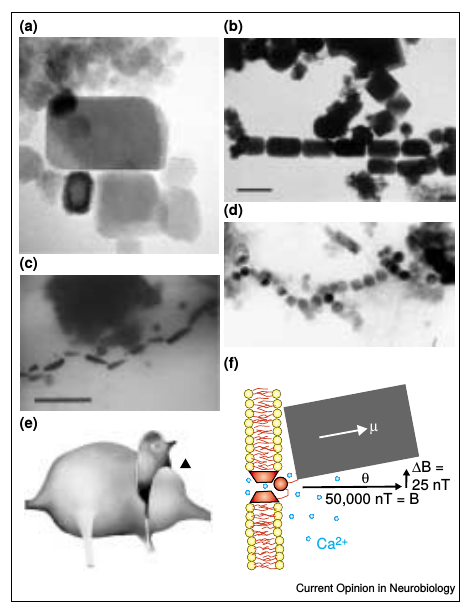
\includegraphics[width=0.5\textwidth]{kirsh2001}
\caption{Magnetosomal mechanism \cite{kirschvink2001magnetite}.}
\label{fig:magnetosome}
\end{figure}

In nature, many organisms have a sense of magnetoreception used for navigation, from magnetotactic bacteria to birds. Two mechanisms have been proposed: a spin-selective (and thus field-sensitive) chemical reaction rate, or magnetite crystals which are actuated by external fields and activate ion channels in the cell membrane (Figure \ref{fig:magnetosome})\cite{johnsen2005physics,dodson2013radical,kirschvink2001magnetite}. Measurements of these magnetosomes show a magnetic dipole moment of up to 100fA/m$^2$ \cite{hanzlik2002pulsed,eder2012magnetic}.

\subsection{Biomimetic sensor design}

Our approach is to mimic the approach found in magnetosomes, with some key modifications so that it is frequency-selective and functions inherently as a gradiometer and thus does not require shielding. The closest biomimetic sensor is a flow sensor which uses ferromagnetic cilia to detect microfluidic flow rates \cite{alfadhel2014magnetic}.

To accomplish this, we propose layering a permanent magnetic layer on top of piezoelectric cantilevers. The torque induced on the magnetic layer generates stress in the piezo layer, and thus a voltage and charge. For an estimate of the sensitivity of this type of sensor, we perform a basic analysis. The moment $N$ induced on the magnetic layer with moment $\vec{m}$ and field $\vec{B}$ is:

$$  N=\vec{m} \times \vec{B} $$

Interpreted as a point load ($N/L$) at the cantilever tip, this moment causes a stress distribution on a cantilever of length L, thickness t, second moment I, piezoelectric voltage constant $g_{31}$, and modulus E, at point (x,y), of

$$ \sigma=\frac{Ny(L-x)}{LI} $$

and $n$ in series generates a voltage

$$ V=\frac{\int_0^L\int_{-t/2}^{t/2}\left|\frac{Ny(L-x)}{LI}g_{31}n\right|dydx}{L} $$


Two features are possible from the cantilever design: frequency selection and gradiometery. As in \cite{shen2008design}, a cantilever has a resonant frequency, which can be modified through geometrical parameters. Peak response will be achieved at this frequency. By selecting many cantilevers of different dimensions, each corresponding to a separate output, the magnetometer output is a spectrometer. Many cantilevers at the same resonance in series generate a larger voltage; in anti-series, the difference is taken, thus functioning as a gradiometer with very high spatial resolution (Figure \ref{fig:diagram}).

\begin{figure}[H]
\centering
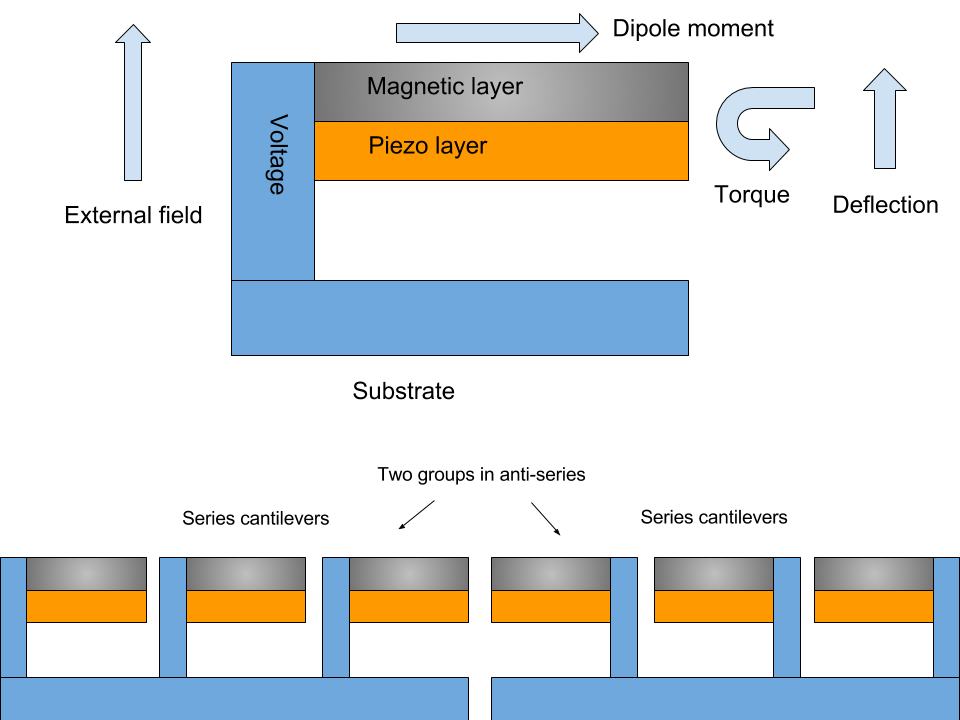
\includegraphics[width=0.7\textwidth]{biomag}
\caption{Diagram of proposed design.}
\label{fig:diagram}
\end{figure}

The noise floor of magnetic materials is governed by Barkhausen noise - the random flipping of magnetic domains \cite{butta2012sources}; this noise is characterized as a flux noise level. The flux noise can be converted into a magnetic moment noise, and thus moment noise. Piezo noise floor is largely a function of piezo losses \cite{levinzon2004fundamental}. Additionally, there is the noise of the amplifier. With conservative estimates for all of these, and two anti-series banks of 30 cantilevers each with dimensions 400x40x3$\mu$m, using a simplified model for a cantilever beam, the sensitivity level is less than 10 fT/cm/$\sqrt{Hz}$, and roughly 100 pT/$\sqrt{Hz}$. Of course, this is an optimistic estimate, and more detailed analysis will be performed when the project starts. 

 Even though biological magnetoreception is limited to nT sensitivity, our design will allow us to surpass this. First, by careful selection of materials (such as Co-Pt or rare-earth magnets) \cite{coey2010magnetism, arnold2009permanent} we can have much higher magnetic dipole moment, and thus higher moment. Second, by careful selection of geometry, we can employ parametric resonance \cite{van2006resonant}. Third, by using many elemens in series and summing, we can increase signal-to-noise ratio (SNR). Finally, using two banks of series cantilevers in anti-series, we both boost the voltage and create a high resolution gradiometer.

 Some potential pitfalls include effects of viscous damping (limiting mechanical vibration at resonance), demagnetization factor (due to the particular geometry of the magnetic layer), and layer separation from stress differentials (if strain at the interface between layers is not equal, they can peel apart). To assess these more closely, multiple physical effects with non-linear, anisotropic materials must be considered simultaneously with a complex geometry. A large part of the MEMS sensor design process must therefore be completed in simulation, allowing us to determine the impact and trade-offs of the above effects before fabrication. Additionally, we can optimize the geometry and material selection for maximum response. Key design variables include the coercivity and remanance of the magnetic layer, the piezoelectric coefficients of the piezoelectric layer, the Young's modulus of each, and the length, width, and thickness of the cantilever. The physics of the system can be described by the PDEs for magnetostatics, mechanical deformation, and the piezoelectric constitutive relations:

 $$ \nabla \vec{B} = 0$$

 $$ \vec{B} = \mu_o(\vec{H}+\vec{M}(\vec{H}))$$

where $\vec{B}$ is the magnetic flux,$\vec{H}$ the sum of external and internal fields, and $\vec{M}$ the magnetization.
 
 $$ -\nabla\cdot\vec{\sigma}=\vec{f}$$
 
 $$ \vec{\sigma} = \lambda(\nabla\cdot u)I+\mu(\nabla u +(\nabla u)^T)$$

 $$ \vec{f} = -\nabla\times\vec{N}$$
 
$$ \vec{N} = \vec{m} \times \vec{B_{ext}}, \vec{m} = \vec{M} $$

where $\vec{N}$ is the moment per volume, $\vec{f}$ is force per volume, $\vec{u}$ is displacement of the beam, $\lambda$ and $\mu$ are Lame elasticity parameters, $\vec{m}$ is magnetic moment per volume, and $\vec{\sigma}$ is the stress tensor.

Finally, to relate field $\vec{E}$, strain $\vec{S}$, displacement field $\vec{D}$, and stress $\vec{\sigma}$, in the piezo layer:
 $$S_{ij} = s_{ijkl}\sigma_{kl}+d_{kij}E{k}$$

$$D_i=d_{ikl}\sigma_{kl}+\epsilon_{ik}E_{k}$$
 
Together, these relations allow us to estimate resonance, stress, and sensitivity of our sensor. COMSOL is one finite-element solver capable of simulating  this structure; another is FeniCS \cite{dupont2003fenics}.


\subsection{Microfabrication process}
Microfabrication processes are capable of constructing the above-described sensor. The process consists of two main fabrication tasks: piezoelectric cantilever construction and magnetic material integration. Zinc oxide (ZnO) has a high strain-to-voltage coefficient in both the 31 and 33 directions and is highly suitable for piezoelectric sensors \cite{tadigadapa2009piezoelectric}. It is also bio-compatible, and environmentally friendly. ZnO is typically deposited with sputtering or solution-based deposition techniques \cite{znaidi2010sol} and patterned with chemical or ion etching.

Rare-earth magnetic materials, such as alloys of Sm-Co, offer high magnetic energy products at room temperature and can be integrated into MEMS using sputtering or pulsed laser deposition (PLD)  \cite{arnold2009permanent}. However, patterning of these materials is slow, using wet etching or ion-beam milling. Additionally, thick films or high aspect ratio structures composed of these materials become difficult, mainly due to the lack of a suitable electroplating process. To solve this problem, it is possible to embed a rare earth transition metal magnetic material, such as NdFeB, in a resin, then use a mold to pattern the magnetic resin composite \cite{wang2013resin}. Additionally, transition metal magnetic materials, such as FePt or CoPt, can be electroplated and also show relatively high magnetic energy products at room temperature \cite{arnold2009permanent,chin2000permanent}.


\begin{figure}[H]
\centering
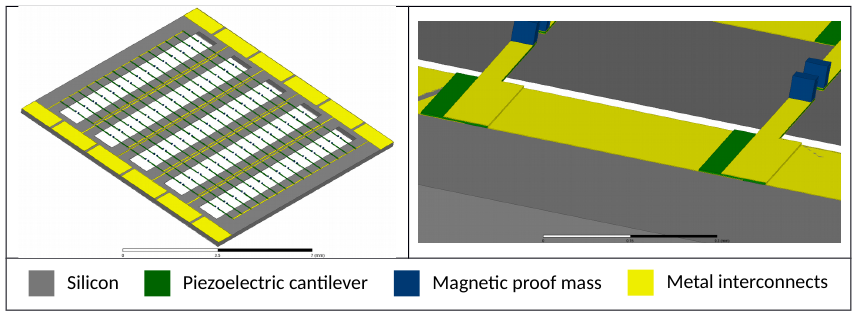
\includegraphics[width=0.95\textwidth]{yoon_3d}
\caption{(Left) 3D view of the entire sensor array (15 x 5). The columns, left facing and right facing cantilevers, are individually addressed and the unconnected terminals (top and bottom corners) are ground. The ground interconnects are not shown to not simplify the image. (Right) 3D close up view of the cantilevers, which are connected in series on each column.}
\label{fig:yoon_3d}
\end{figure}

\begin{figure}[H]
\centering
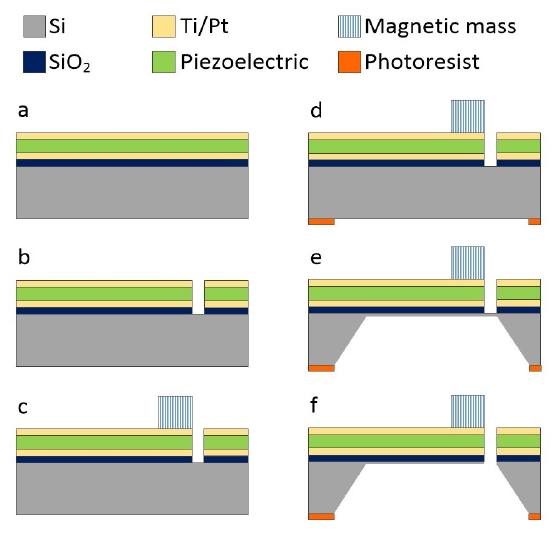
\includegraphics[width=0.5\textwidth]{yoon_process}
\caption{Magnetic cantilever fabrication. Though pictured with a magnetic proof mass, this could also be used with a magnetic layer. The patterning associated with steps 1-3 of the process described in the text are not shown due to image complexity and are represented by (a).}
\label{fig:yoon_process}
\end{figure}

Our proposed fabrication procedure for the sensor pictured in Figure \ref{fig:yoon_3d} is similar to others in MEMS \cite{shen2008design}. The process involves six masks with one being a backside mask. The process will require double sided polished wafers, but the p+ etch stop removes the need for SOI wafers. However, if the doping process does not give the needed uniformity, SOI wafers may be used as well. Alternatively, if the KOH etching is too rough or if smaller spacing between columns is needed, reactive ion etching (RIE) may be used for the backside etch. The electrode area is patterned separately from the cantilevers since the accuracy of both the alignment and etching is not nearly as high. The detail fabrication steps are as follows:


\begin{enumerate}
\item Deposit silicon oxide using plasma enhanced chemical vapor deposition (PECVD) and pattern bottom electrode materials (titanium and platinum: Ti/Pt) with RIE etching according to the first mask in the electrode area (Fig. \ref{fig:yoon_process}(a))
\item Deposit the piezoelectric material (ZnO) and pattern with wet etching according to the second mask in the electrode area (Fig. \ref{fig:yoon_process}(a))
\item Deposit the top electrode material (Ti/Pt) and pattern with liftoff according to the third mask in the electrode area (Fig. \ref{fig:yoon_process}(a)) 
\item Use RIE to etch the layers deposited in the preceding steps to define the cantilever with the fourth mask (Fig. \ref{fig:yoon_process}(b))
\item Deposit the magnetic proof mass or layer using the mold approach (NdFeB) or electroplating (FePt or CoPt) with the fifth mask (Fig. \ref{fig:yoon_process}(c))
\item Use backside exposure to pattern the backside of the silicon according to the sixth mask (Fig. \ref{fig:yoon_process}(d))
\item Etch the backside of the silicon using KOH with a p+ epilayer as an etch stop (Fig. \ref{fig:yoon_process}(e))
\item Release the cantilevers with a selective frontside RIE (Fig. \ref{fig:yoon_process}(f))
\end{enumerate}
\subsection{Circuit design}
 
From circuits and systems point of view, this could be modeled using a very-large-scale oversampling sensing architecture. A simple example is laid out as follows: 

Assuming a sensor of area $A$ generates a signal of $S$, and it has intrinsic noise of $N_i$. In comparison, two sensors each with an area of $A/2$ would each generate a signal of $S/2$ and noise of $N_i/2$. When the two $A/2$ sensors are combined, their total signal will be $S$. But since the noises from the two $A/2$ sensors are uncorrelated, the combined total noise will be:

$$\sqrt{(N_i/2)^2+(N_i/2)^2} = N_i/\sqrt{2} $$

Therefore, splitting a sensor into two with equal size will result in a factor of $\sqrt{2}$ increase in the signal-to-noise ratio (SNR). Likewise, splitting a sensor into an array of $M$ small units that sum up to the same total size would lead to a factor of $\sqrt{M}$ increase to the SNR. Because of this “oversampling gain” to the SNR, magnetosomes with thousands of magnetite crystals are able to have a superb sensitivity to small fluctuations of magnetic field, which can hardly be achieved by conventional man-made tools. 

\begin{figure}
\centering
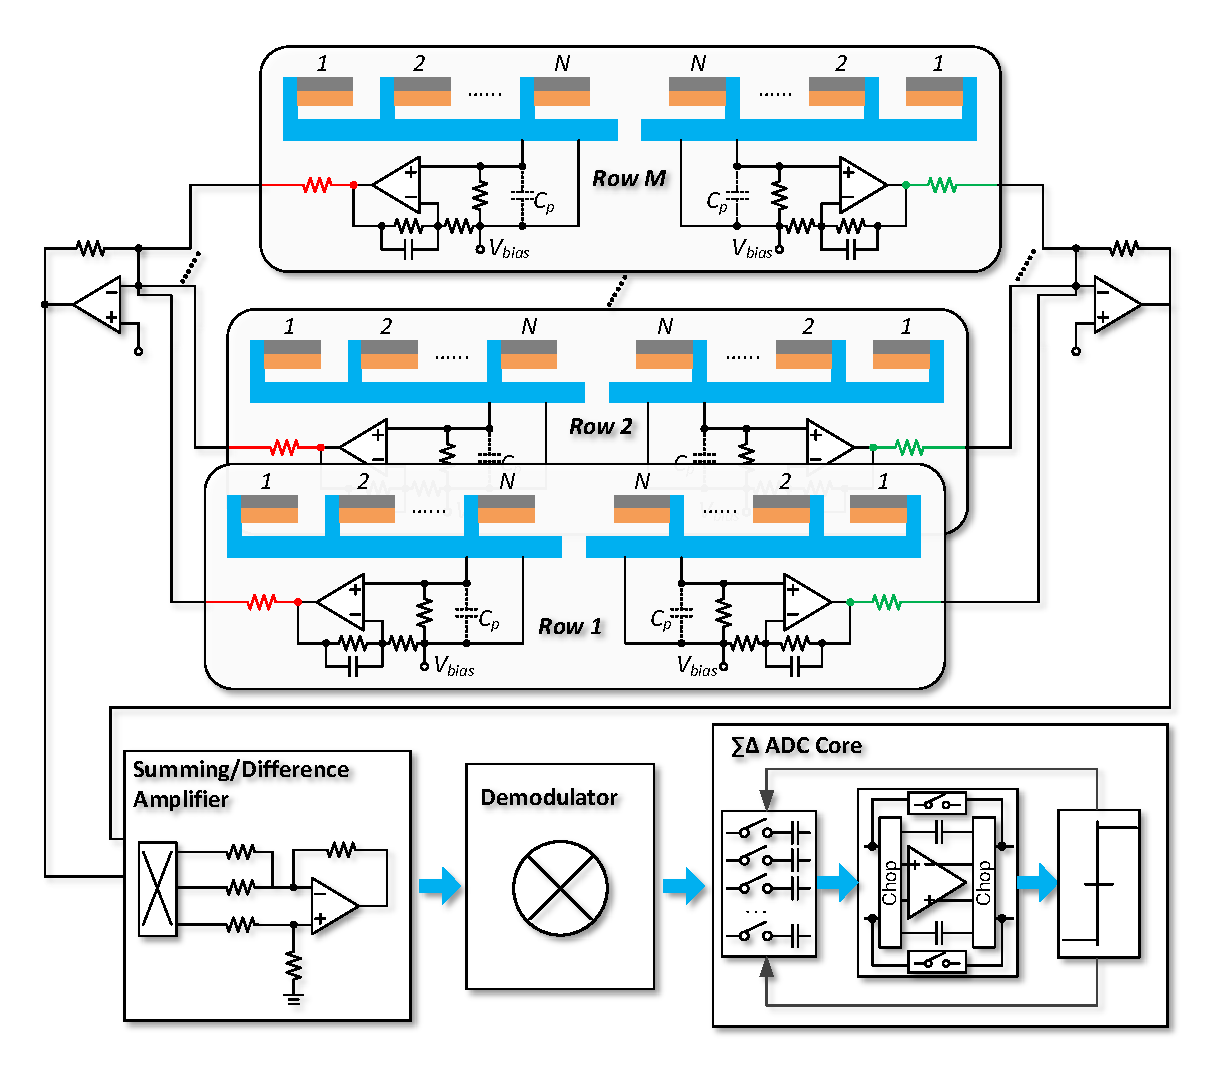
\includegraphics[width=0.65\textwidth]{System}
\caption{System design.}
\label{fig:system}
\end{figure}

Ideally, if a sensor can be split into an infinite number of miniaturized elements, it would approach the capability of magnetosomes to achieve ultra-high field sensitivity. On the other hand, it is the most desirable to implement this bio-inspired oversampling mechanism in the analog front-end because any added back-end circuitry would introduce parasitics and noise that would otherwise hinder the effectiveness of the ideal oversampling theory. Inspired by this bio-mechanism of oversampling, we propose to combine the magnetic/piezo cantilevers in groups, and use low-noise amplifiers to pick up signals directly from the elements. The low-noise amplifiers will be reconfigurable in summing and difference modes to detect total field and field gradient. An overview of the system is shown in Figure \ref{fig:system}.

Voltage-mode and charge-mode amplifications are two main approaches to signal conditioning of piezoelectric sensors. Voltage-mode amplification is useful when the amplifier is very close to the sensor and thus minimal parasitic capacitance is presented by the interconnection between the sensing device and the amplifier input. Charge-mode amplification is useful when the amplifier is remote to the sensor because it is robust against parasitic capacitance of interconnections. Depending on the characterization and optimization of the MEMS device front-end, the team is ready to investigate both approaches and fully integrate the final solution with special circuit techniques for the optimal performance. 

\subsubsection{Voltage-mode approach}

The simplified structure for voltage-mode amplifiers is depicted in Fig. \ref{fig:system}, represented by the circuits that directly interface with each row of the MEMS device. Depending on the fabricated and optimized MEMS size, either one or multiple amplifiers in parallel will be implemented for each row to collect the piezoelectric voltage signal. The goal of using multiple amplifiers in parallel is to enhance the SNR because of the benefit of oversampling. However, constraint exists due to the area available under the MEMS device. The circuit team will work closely with the microfabrication team in this project to determine the ideal placement of local voltage-mode amplifiers in Phase I of this project, and compare the performance with the charge-mode approach discussed next.  

\subsubsection{Charge-mode approach}

\begin{wrapfigure}{R}{0.5\textwidth}
\centering
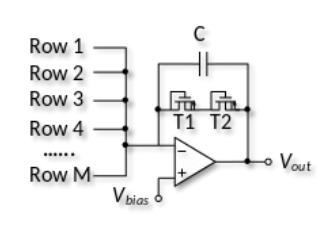
\includegraphics[width=0.4\textwidth]{cmos}
\caption{Charge-mode amplifier with pseudo-resistor feedback and summing capability.}
\label{fig:cmos}
\end{wrapfigure}

Charge-mode amplifier approach will also be investigated because it has advantages in handling interconnect parasitics and the convenience of adding signals from different rows of the MEMS device together. Inspired by existing works in neural recording \cite{harrison2003low}, the team will use MOS-bipolar pseudo-resistors as the feedback resistors in the charge-mode amplifier. As shown in Fig. \ref{fig:cmos}, two back-to-back connected PMOS transistors (T1 and T2) that can easily achieve resistance of several gigaohms will be implemented as the feedback resistor of the charge-mode amplifier, enabling processing brain signals with a frequency as low as 0.025 Hz. With negative VGS, T1 and T2 function as diode-connected PMOS transistors. With positive VGS, the parasitic source-well-drain p-n-p bipolar junction transistor (BJT) is activated, such that T1 and T2 act as diode-connected BJTs. For small voltages across the pseudo-resistors, the small-signal resistance is extremely high and thus moves the corner frequency to low enough for bio-signal processing. On the other hand, a large voltage across the pseudo-resistors will reduce the small-signal resistance and result in a fast settling time for the amplifier. As a result, this pseudo-resistor-based design can amplify low-frequency signals down to the millihertz range while properly rejecting large DC offsets. The theoretical noise-power tradeoff limit, i.e., the noise efficiency factor, have already been derived and demonstrated by selectively operating MOS transistors in either weak or strong inversion \cite{harrison2003low}. The only potential drawback of this configuration is that the amplifier cannot have a large output swing, because otherwise the pseudo-resistors may become two diodes. However, this is not a concern for this work as the amplifier is implemented as pre-amplifier in the front-end, where signal to be handled is very weak.

\subsubsection{Re-configurable summing and difference amplifiers}

After the piezoelectric signal is captured by arrays of preamplifiers located near the MEMS sensors, the obtained voltage signals will be further processed by a re-configurable summing and difference amplifier. This amplifier will be digitally controlled in real-time to either add or subtract signals coming from different regions of the fabricated sensor. This will enable both common-mode detection, which senses the total field, and differential-mode detection, which senses the field gradient.

One potential challenge for the summing and difference amplifier is the tradeoff between high sensitivity and large dynamic range. Being able to perform both summing and difference detection, as well as the existence of strong earth field, requires the amplifier to have a very large dynamic range. However, the DARPA specifications also mandate high sensitivity for brain signal recovery. To this end, a 3-op-amp topology will be customized and implemented in GlobalFoundries 180-nm SiGe BiCMOS 7WL process for both low-noise and high-linearity operation. Bipolar PNP transistors will be utilized as the input buffer to minimize the input-referred noise. A programmable resistor array will be implemented between the outputs of the two first-stage amplifiers to provide a large tunable gain range. In a previous DARPA project (MELD – Mind Electromagnetic Localization Device), the team has evaluated various topologies and different semiconductor processes (e.g., SOI versus BiCMOS) for the amplifier of brain magnetic field detector, and verified through both Cadence simulation and fabricated chip measurement that the 3-op-amp topology with bipolar transistor input buffer offers the best combined sensitivity and linearity performance.

\subsubsection{Solution to low-frequency noise and device mismatch in electronics}

Because the magnetic field induced by brain activity is extremely weak, and contains low frequencies (below 100 Hz), 1/f noise and device mismatch have significant impact to the success of the proposed work. To resolve the challenge, the bio-inspired magnetic sensor will operate at a resonant frequency which “carries” the signal of interest. A double-balanced demodulator featuring low noise at the baseband output, high rejection to harmonic distortion, and low LO/RF leakage will be implemented after the summing/difference amplifier to recover the field information of interest. 

After the signal is demodulated to the baseband, circuit techniques including dynamic offset cancellation, dynamic element matching (DEM), and chopping will be applied extensively to the remaining signal processing circuits to cancel the mismatch errors and low-frequency noises. On the data acquisition side, the analog-to-digital converter (ADC) is an important component for correctly interpreting the field information. Nyquist ADC accuracy is limited by the matching of components in ADCs, while oversampling ADCs, such as sigma-delta ADC, trade speed for resolution. Because brain signals have low frequencies, sigma-delta ADC is a very good candidate for precision sensing. Another advantage of sigma-delta ADC is that chopping technology and dynamic element matching are suitable for its architecture to minimize the impact of low-frequency noise and offset errors.


\section{Risk Analysis and Mitigation Plan}

\begin{table}[h!]
\centering
\begin{tabularx}{.85\textwidth}{|X||c|c|X|}
    \hline
    Risk & Probability & Impact & Plan\\
    \hline
    \hline
    Insufficient sensitivity in simulation & 5 & 10 & Optimize design architecture. \\
    \hline
    Best available MEMS processes infeasible & 4 & 10 & Begin design process within constraints of available processes. \\
    \hline
    Interconnects infeasible & 3 & 5 & Operate fewer, larger cantilevers \\
    \hline
    Viscous damping hurts sensitivity & 5 & 7 & Operate in vacuum packaging \\
    \hline
    Resonance frequency too high & 6  & 10 & Operate fewer, larger cantilevers, or operate off-resonance \\
    \hline
    Fabrication mismatch & 3 & 5 & Begin fabrication early, so process can be adjusted; dynamic element matching. \\
    \hline
    Sensitive to mechanical vibration & 3 & 5 & Use additional, non-magnetic cantilevers to cancel mechanical vibrations. \\
    \hline
    Insufficient torque generated on magnetic substrate & 5 & 10 & Re-evaluate material selection and geometery. \\
    \hline
\end{tabularx}
\caption{Risk matrix}
\label{table:risk}
\end{table}

Since this is a novel design, there is not a benchmark design in the literature which we know a priori is achievable. There are several risks and challenges associated with this design, many of them impactful on the probability of success. Most can be addressed early, simply by doing careful analysis of the problem within the range of constraints on materials and processes. Others (the density of interconnects, or resonant frequency being too high) can be addressed by reducing the number of elements and increasing their size. Damping, due to the viscosity of air, may hurt sensitivity and could be addressed by vacuum packaging the sensor head. Manufacturing mismatch of the sensing elements can be effectively removed by dynamic element matching, where the transducers are switched electronically to average out fabrication differences.

Mechanical redundancy will be employed to mitigate some problems that will arise in fabrication that will affect the quality factor (Q), e.g. mismatch, stress gradients across wafer, and contaminates. This redundancy is achieved by making many cantilever sensors connected in parallel, and then selecting desired ones. For sensor selection, a single cluster of devices will be probed, swept in frequency, and their individual frequency response characterized via laser doppler velocimetry (LDV) to find bandwidth and resonance frequency.  Devices with at least a 3dB overlap of resonance frequency to bandwidth will be chosen and remaining unwanted devices will be discarded either by cutting the electrical connection or physically removing free standing beam.

\section{Schedule and Milestones}

\begin{figure}[H]
\centering
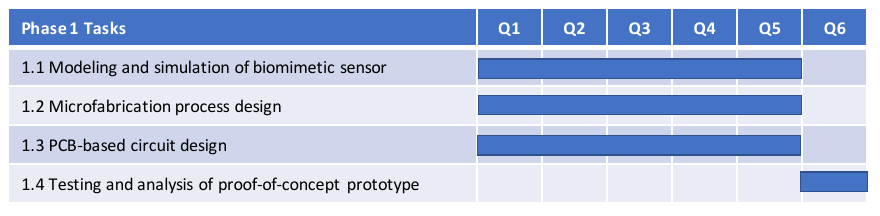
\includegraphics[width=\textwidth]{Gantt1}
\label{fig:gantt1}
\end{figure}
Phase 1 Milestones:
\begin{itemize}
\item End of Q5: complete modeling and design of biomimetic sensor; complete microfabrication plan and sensor prototype;
complete PCB circuit.
\item End of Q6: demonstrate the proof-concept prototype meeting Phase 1 requirements.
\end{itemize}


\begin{figure}[H]
\centering
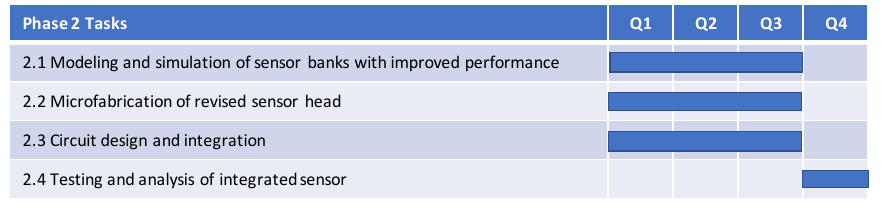
\includegraphics[width=\textwidth]{Gantt2}
\label{fig:gantt2}
\end{figure}
Phase 2 Milestones:
\begin{itemize}
\item End of Q3: complete simulation and design of sensor banks with improved performance; complete microfabrication
of revised sensor head; complete sensor amplification IC.
\item End of Q4: demonstrate the integrated sensor meeting Phase 2 requirements.
\end{itemize}

\begin{figure}[H]
\centering
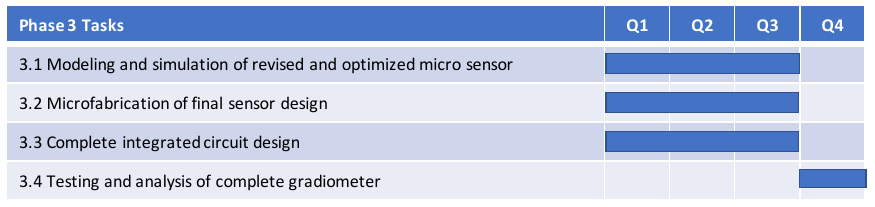
\includegraphics[width=\textwidth]{Gantt3}
\label{fig:gantt3}
\end{figure}
Phase 3 Milestones:
\begin{itemize}
\item End of Q3: complete simulation and design of final optimized micro sensor; complete design and fabrication of
sensor amplification IC with ADC; complete fabrication and integration of final sensor with IC.
\item End of Q4: demonstrate the final gradiometer meeting Phase 3 requirements.
\end{itemize}

\section{Test Plan}\label{sec:test}

To test, in Phase 1, the sensor will first be connected to the circuitry and powered to establish basic functionality.  Prior to testing, noise from the Helmholtz coils, power supplies, and any other necessary signal generation sources will be characterized. Further, the sensor will be placed in a pair of Helmholtz coils driven with precision current sources, inside a magnetic shield, so we can gauge accuracy and sensitivity in a controlled environment. Field gradient, intensity, and frequency will be swept over the range specified in Table \ref{table:obj}. Finally, the same test will be repeated in an unshielded environment. In each case, we will monitor power consumption and signal output, and measure sensor and control electronics volume. Subsequent phases will follow a similar testing protocol, except using specifications for those phases. Additionally, in Phases 2 and 3, where an IC will be developed and integrated with the sensor head, the IC will be tested independently to verify basic input/output functionality before slicing and bonding to the MEMS substrate.

\section{Results and Technology Transfer}

Our research team has demonstrated successful technology transfer to the government and private sectors in our work on wireless power, vital signs radar, and low-field magnetometry. UF's Office of Technology Licensing is very helpful in patenting and licensing new engineering developments from research. Dr. Lin's group produced several patents on wireless power and wireless sensor that have already been licensed. The technology transfer of wireless charging technologies to WiPower resulted in a successful acquisition by Qualcomm. Dr. Yoon's group has developed a smart mouthguard, as a wearable biomedical device for health monitoring. The technology is in a license option agreement phase with Dentsply-Sirona Inc., a dental supplier and instrument company. Dr. Li's group has full support from the TTU Office of Research Commercialization on technology transfer. Several IPs developed by Dr. Li's group on biomedical radar sensors are licensed to startup company yearONE, LLC.

This project based on innovative biomimetic concept is expected to generate intellectual properties (IP) on sensor design, microfabrication process, and circuit design that can be patented and licensed to companies interested in commercialization. The team will work with their universities on patent application and technology transfer as soon as any new IP is generated. 

\section{Ongoing Research}
Current state of the art magnetometers include the standard, cryogenic SQUID \cite{lenz2006magnetic}. The novel spin relaxation free magnetometer has been minaturized and achieves less than 10 fT/$\sqrt{Hz}$, but still requires shielding and lacks directional sensitivity \cite{shah2013compact}. Fluxgates have achieved pT level resolution at small size, but this is insufficient for biomagnetic field measurement \cite{sasada2002orthogonal,uchiyama2014highly,sasada2014fundamental}. Lorenz-type magnetometers, which translate magnetic fields into mechanical actuation of a magnet or current carrying wire, have been built in MEMS substrates, but have insufficient sensitivity and require shielding \cite{sinha201627,kyynarainen20083d,kumar2015ultra,thompson2009parametrically}.

\section{Proposer Accomplishments}
Drs. Lin, Li, and Casanova were involved in a previous DARPA project for detection and inversion of MEG/EEG signals. They have worked on all phases, from sensor design to circuit design to inversion algorithm. Additionally, Drs. Lin and Li have collaborated extensively on vital sign radar, and Dr. Casanova has worked on electromagnetic sensors for agriculture and analytical chemistry. Dr. Yoon has conducted research on microfabrication of MEMS-based sensor systems using piezoelectric and magnetic materials. He is currently working on a DARPA M3IC project as a Co-PI.

\section{Facilities}
UF and TTU have adequate facilities to carry out the proposed research tasks.
PI Lin's facilities at UF for sensor development and testing include magnetic shielding, circuit testing instrumentation (power supplies, oscillopes, function generators, vector network analyzer). Co-PI Yong-Kyu Yoon is a member of the Interdisciplinary Microsystems Group (IMG) laboratories at UF that consist of 11 newly renovated laboratories with 5800 ft$^2$ of lab space used for microsystems design, fabrication, packaging, and characterization.  Seven lab spaces (computer, machine shop, electrical testing, mechanical testing, optics, packaging, and wet processing) are considered to be communal lab spaces and the remaining four labs contain more specialized equipment for specific areas of research. Also, an additional simulation lab in the ECE department is located in New Engineering Building (NEB) 500. Available software includes following: PSpice (OrCAD Inc.), Multiphysics simulation tool COMSOL package (COMSOL Inc.), and  High frequency structure simulator (HFSS, Ansys, Inc.), among others. The electronic characterization facility contains an impedance Analyzer (HP 4194),  spectrum analyzer,  vector network analyzer (Agilent, E5071E) (3 kHz ~ 20 GHz), and a probe station (Cascade Microtech).

The UF Nanoscale Research Facility (NRF) is a multi-user oriented class 100-1000 cleanroom facility that provides nanofabrication and characterization equipment to the scientific community at the University of Florida. The cleanroom features a bay-and-chase layout with seven different research bays, including e-beam lithography, photolithography, wet processing, hot processing, thin film deposition, and dry etching bays.  Additionally, electroplating systems for copper and ferromagnetic materials and high temperature furnace (Linderburg) are available in BEN 230 and 237C. Major device fabrication equipment includes: Raith-150 electron beam direct write lithography system, deep UV photolithography system, EVG 620 back-side aligner/wafer bonder, Karl Suss MA6, MJB3 aligners, EVG501 wafer bonder, STS 310PC PECVD, KJL multi-target sputtering system, E-beam and thermal evaporators Tystar LPCVD, oxidation, polysilicon, and diffusion furnaces, STS ASE deep reactive ion etcher, Unaxis RIE-ICP, dicing saws, wire-bonders, and die bonding apparatus, as well as metrology instrumentation.

Dr. Li's research group at the Texas Tech University is located in a fully ESD-protected Microwave and Analog Circuits Laboratory. The PI has obtained full support from the Texas Tech University Provost Office and Electrical and Computer Engineering Department to establish this well-equipped lab and enhance the department’s research strength on the microwave, and analog circuits. Equipment includes high-frequency network analyzers, signal generators, spectrum analyzer, and oscilloscopes; software useful to this project includes Cadence, Altium, MATLAB, and Labview.

\section{Teaming}
The project team consists of Dr. Jenshan Lin, Dr. Joaquin Casanova, and Dr. Yong-Kyu (YK) Yoon from University of Florida, and Dr. Changzhi Li and Dr. Scott Block from Texas Tech University. While working on the previous DARPA project, Dr. Lin teamed up with his former Ph.D. students Dr. Casanova and Dr. Li to work on the design of room-temperature MEG sensors and circuits for unshielded operation as well as the inversion algorithm for signal processing. Toward the end of the project, an idea of this proposed biomimetic sensor emerged as a promising candidate to significantly improve the sensitivity in unshielded environment while significantly reducing the size. The new concept requires microfabrication using thin-film magnetic materials and piezoelectric materials, and therefore Dr. Lin invited his colleague Dr. Yoon, an expert on this specific microfabrication process, to join the team. Dr. Lin and Dr. Yoon have served several times on each other's Ph.D. student committees, and are familiar with each other’s technical expertise.

In this project, Dr. Lin will serve as the PI managing the project. Dr. Lin is currently serving as a program director of Communications, Circuits, and Sensing Systems in National Science Foundation. His two-year appointment is scheduled to end on 10/18/2018. While at NSF, he is allowed to spend about 20\% his time on university research projects (but no salary support on government-funded projects per NSF rule). Dr. Lin is planning to dedicate 10\% effort on this proposed project in the first 12 months, end his NSF appointment earlier to return to his university position on 10/1/2018, and switch to 15\% effort on this project during academic semesters and 33\% effort during summer. The project management during the first 12 months is not a problem, as in the pervious DARPA project he also served as the PI and Dr. Casanova handled all technical matters while he was away at NSF. The same arrangement is expected to work, and therefore Dr. Lin and Dr. Casanova are both listed as Technical Point of Contact. 

With the experience on a relevant project as well as past working relationships and complementary expertise areas among members, the team is well suited to execute this project. Details of the expertise and task assignment of each team member are listed below. 

\begin{description}
  \item[Jenshan Lin] Project Lead overseeing all tasks on this project and co-supervise a graduate student and an undergraduate student with Dr. Casanova. 10\% (0\% in budget) 10/1/2017-8/31/2018, 15\% academic months/33\% summer months starting 10/1/2018. He received Ph.D. in Electrical Engineering from UCLA in 1994, and worked for Bell Labs (under AT\&T and Lucent) and its spinoff Agere Systems 1994-2013. He has been a faculty in University of Florida since 2003, and is currently a Full Professor. He is a Fellow of IEEE, and is an expert on RFIC, wireless sensors, and wireless power transfer. He has over 260 technical publications in refereed journals and conference proceedings, and holds 15 patents. Since joining University of Florida, he has graduated 24 Ph.D. students.
  \item[Joaquin Casanova] will conduct electromagnetic simulation and design of the MEMS sensor, and work with Dr. Yoon on process/material selection, and Dr. Li on requirements for the interface and control circuits. His commitment is 25\% academic months/33\% summer months starting 10/1/2017, and 15\% academic months/33\% summer months in Phase 2 and 3. He received a B.S. and M.E. in Agricultural and Biological engineering in 2006 and 2007 from UF, and PhD in Electrical Engineering in 2010 from UF. His work has primarily focused on sensors and electromagnetic design, including wireless power, microwave remote sensing, agricultural sensors, analytical chemistry equipment design, and low-field magnetic sensing. He is currently a Research Assistant Professor in UF's Department of Electrical and Computer Engineering. 
  \item[YK Yoon] will guide selection of a microfabrication process and fabrication of the sensor. Collaborating with Dr. Lin, Dr. Casanova, and Dr. Li, he as a Co-PI supervises two graduate students for microfabrication of sensors. He commits his efforts for 15\% academic months and 33\% summer months through out all the phases. He received his Ph.D. degree in electrical and computer engineering from the Georgia Institute of Technology, Atlanta, GA in 2004. He is currently an Associate Professor in the Department of Electrical and Computer Engineering at the University of Florida, Gainesville, FL. He has direct experience in the development of MEMS resonator based magnetic sensors \cite{choi2006magnetically, choi2006magnetically2, choi2011nonlinear}, and strong expertise in microfabrication \cite{yoon2006multidirectional}, piezoelectric \cite{wulateral}, ferroelectric \cite{kim2014microwave,yoon2005low,yoon2003reduced}, ferromagnetic \cite{rahimi2016study,rahimi2015cylindrical,yoon2013multi}, and multiferroic devices \cite{yoon2013multi,kim2014room}.

  \item[Changzhi Li] will design the electronics for amplifying and digitizing the signals from the sensor head, working with Dr. Casanova to determine circuit requirements. His time commitment is 15\% academic year and 1 summer month. He received the B.S. degree in electrical engineering from Zhejiang University, China, in 2004 and the Ph.D. degree in electrical engineering from the University of Florida, Gainesville, FL, in 2009. In the summers of 2007 and 2008, he worked at Alereon Inc., Austin, TX, on ultrawideband (UWB) transceiver. In the summer of 2009, he worked at Coherent Logix Inc., Austin, TX, on software-defined radio. He was a consultant for DIS Semiconductor in Austin, TX in the summer of 2012. He was a consultant for Texas Instruments (TI) teaching TI employees 'Design \& Analysis of Analog ICs in LBC7 Process' in the summer of 2013. His research interests include analog circuits, microwave circuits, and biomedical applications of microwave/RF. He has published over 200 journal and conference papers in these fields. He holds 6 US patents.
  \item[Scott Block] received his B.S. in Mechanical Engineering from the University of Illinois at Urbana- Champaign in 2006, M.S. degree in Electrical Engineering from Texas Tech University in 2010, and PhD degree in Electrical and Computer Engineering from the University of California at Davis in 2017. He has held internship positions at MEMS startup companies Chirp Microsystems (ultrasonic gesture systems) and Picosense Inc. (magnetic sensing of the heart). His research interests include mixed-signal CMOS circuit design, MEMS, W-to-nW sensor interfaces, energy harvesting, and power electronics. He designed, fabricated, and tested 3 different versions of nW mixed signal front-ends for MEMS microphones and accelerometers used as a trip sensor for UC Davis’ entry to the N-ZERO DARPA project. He also contributed heavily to the proposed design for Phase 2 of the N-ZERO project. Dr. Block is relocated to Lubbock TX and will serve as a research associate for the proposed AMBIENT project.
  
\end{description}
\newpage
\required{Section III: Additional Information}

\bibliography{./casanova_ieee}
